\documentclass{beamer}

\usetheme{Copenhagen}

\title{A Prolog interpreter for the browser}
\author{William Henderson}
\institute{Churchill College \\
University of Cambridge}
\date{Thursday 13th February 2025}

\begin{document}

\frame{\titlepage}

\begin{frame}
\frametitle{Motivation}

\begin{itemize}
\item Prolog is widely used on the Web, but current implementations are lacking:
\begin{itemize}
\item Client-server: require a server.
\item \emph{Web-ported}: lack browser integration.
\item \emph{Web-native}: JavaScript is slow.
\end{itemize}
\end{itemize}

\vspace*{5mm}

\begin{block}{Question}
\textbf{Can a web-native Prolog implementation, targeting WebAssembly, do better than existing solutions?}
\end{block}

\end{frame}

\begin{frame}
\frametitle{Project Status}

\begin{itemize}
\item Success criteria met:
\begin{itemize} 
\item[\checkmark] \textbf{Prolog implementation built} in Rust, compiled to WebAssembly, and running in the browser.
\item[\checkmark] \textbf{Performance evaluated} against existing solutions.
\item[\checkmark] Key \textbf{optimisations made} to improve performance.
\end{itemize}

\item Extensions completed:
\begin{itemize}
\item[\checkmark] \textbf{Precise garbage collector}, incl. variable shunting, early reset.
\item[\checkmark] \textbf{Web-based Prolog development environment} built.
\item[\checkmark] \textbf{Inline JavaScript FFI} for browser integration:
\end{itemize}
\end{itemize}

\vspace*{2mm}

\begin{center}
\texttt{add(X, Y, Z) :- <\{ (X, Y, Z) => unify(Z, X + Y) \}>}
\end{center}

\end{frame}

\begin{frame}
\frametitle{Web-Based Development Environment}

\begin{center}
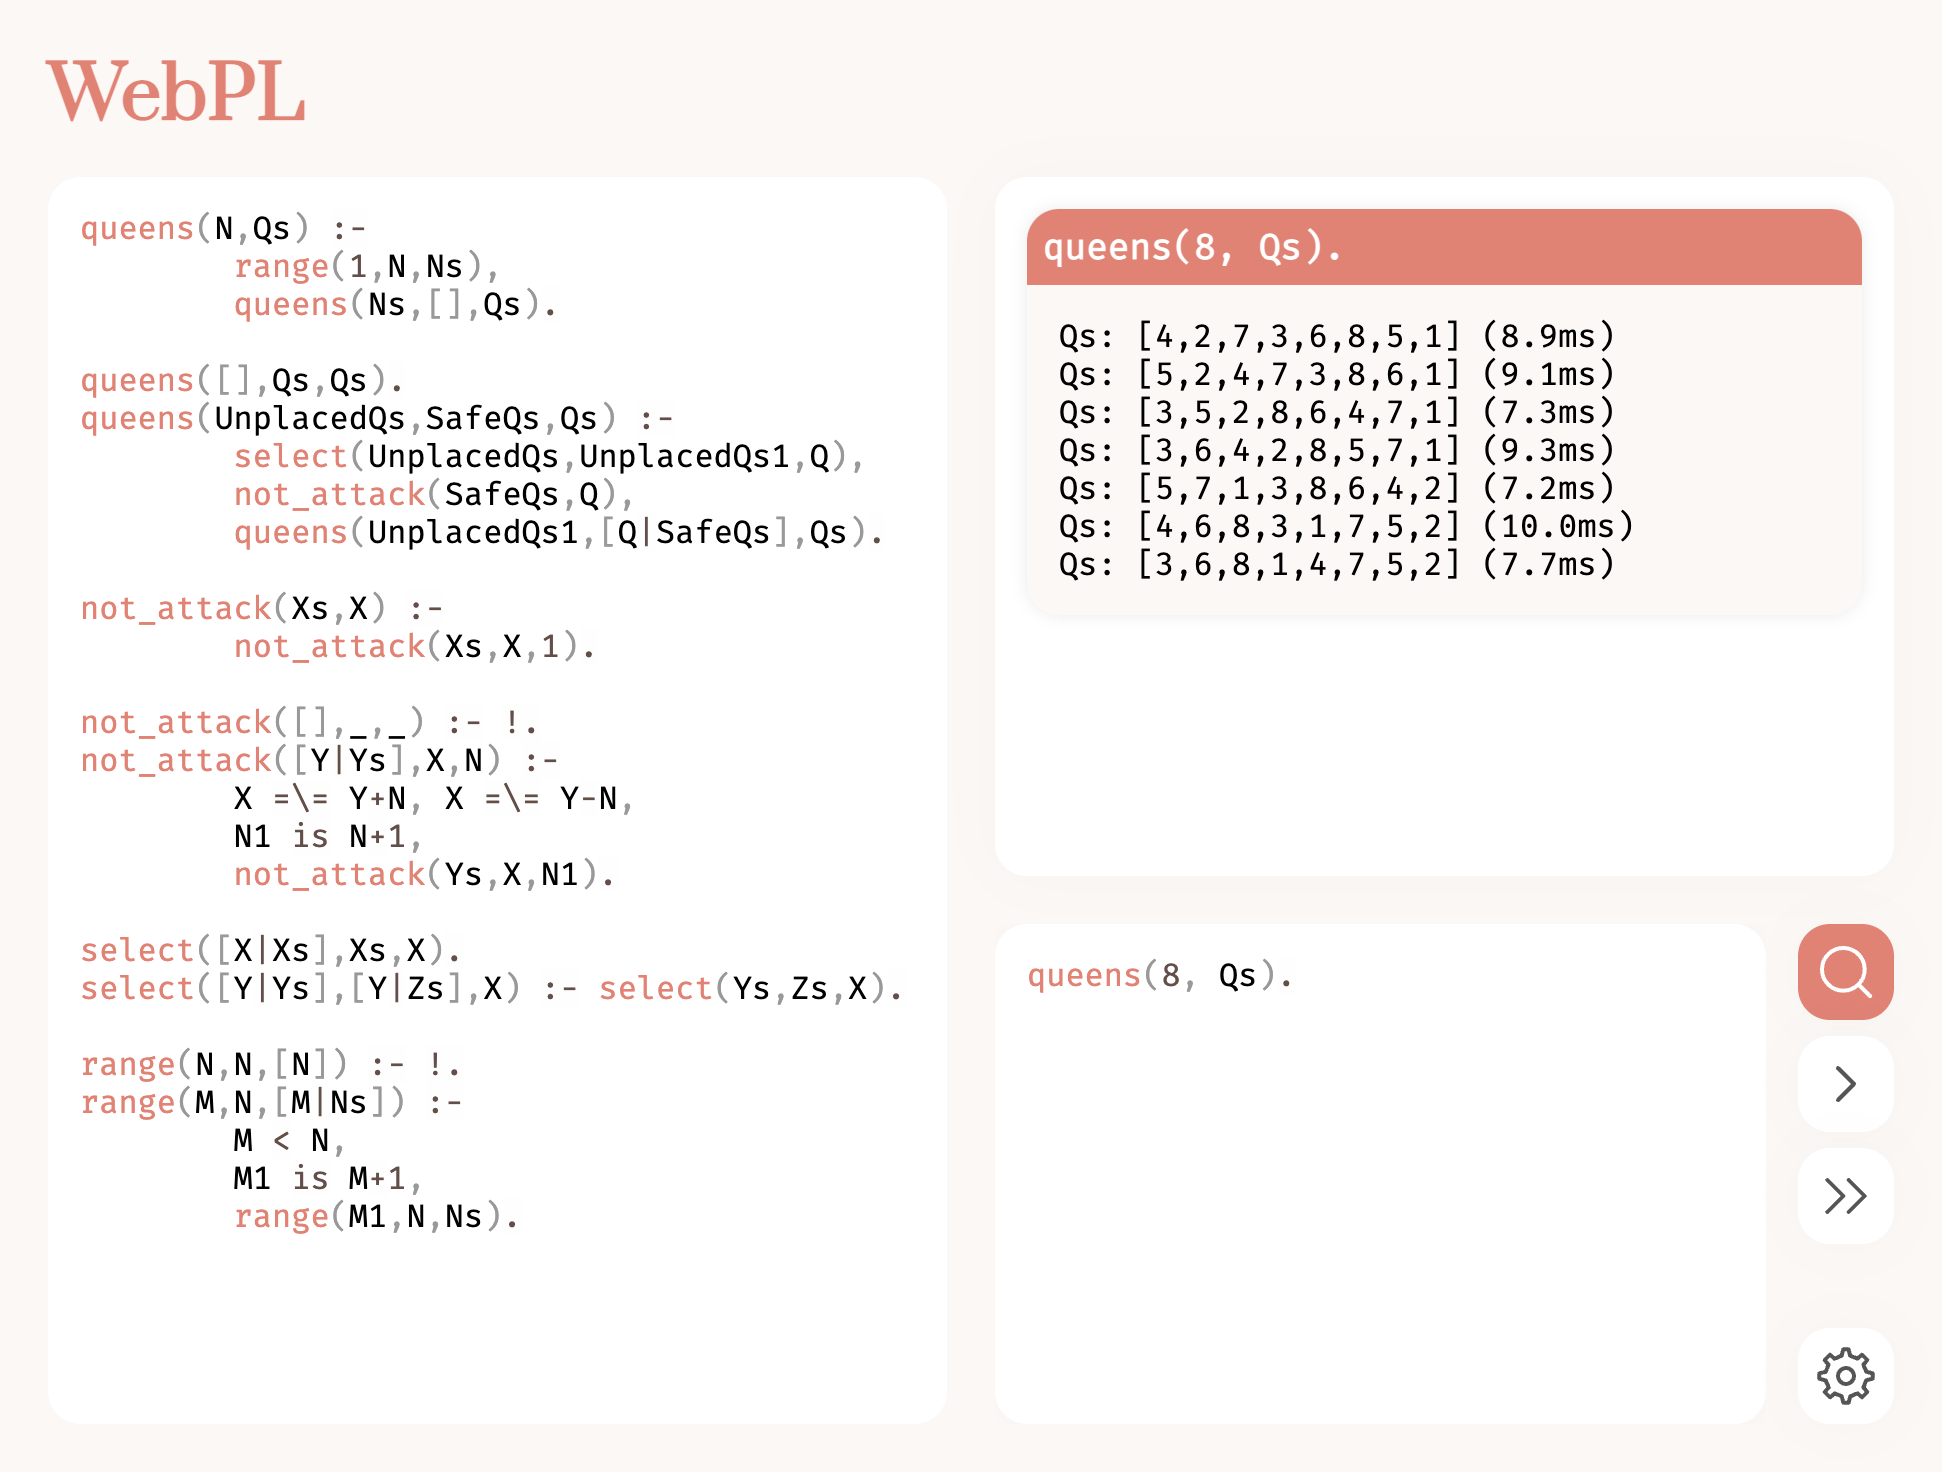
\includegraphics[width=0.85\textwidth]{browser.png}
\end{center}

\end{frame}

\begin{frame}
\frametitle{Benchmark Results}

\begin{figure}[h]
\centering
\begin{minipage}{0.45\textwidth}
  \centering
  \includegraphics[width=\textwidth]{execution.pdf}
\end{minipage}
\hfill
\begin{minipage}{0.45\textwidth}
  \centering
  \includegraphics[width=\textwidth]{memory.pdf}
\end{minipage}
\end{figure}

\end{frame}

\begin{frame}
\frametitle{Remaining Work}

\begin{itemize}
\item Optimise garbage collection further.
\begin{itemize}
\item Improve scheduling to minimise overhead
\item Explore other GC algorithms (e.g.\ copying, generational)
\end{itemize}
\item Fix bugs in the web-based development environment.
\item Extend the JavaScript FFI to support more complex terms and operations, maybe taking an object-oriented approach.
\end{itemize}


\end{frame}

\end{document}